%%
The leading twist tensor structure function $b_1$ quantifies effects not present in 
the case of spin-1/2 hadrons. However, tensor effects only
exist in nuclear targets, so the study of $b_1$ serves as a very interesting bridge between nucleon and nuclear physics.
On the one hand, deep inelastic scattering (DIS), clearly probes partonic degrees of freedom, i.e. quarks, but on the 
other hand, $b_1$ depends solely on the deuteron (nuclear) spin state as seen in Eq.~\ref{TSF-parton}. We discuss now several predictions for the $x$ dependence of $b_1$.

%A measurement of $b_1$ would allow us to take 
%a deeper look at the nucleus internal dynamics, since $b_1$ should be zero if the 
%nucleus is made up of spin-1/2 constituents at rest, or in a relative $s$-wave. 
%Therefore a non-negligible value of $b_1$ can be understood in terms of the deviation 
%of a nucleus from a simple bound state of protons and neutrons, 

%
\subsubsection{Conventional Nuclear Effects}
%\subsubsection*{Hoodbhoy, Jaffe and Manohar}
In Ref.~\cite{Hoodbhoy:1988am}, the authors note that $b_1(x)$ is small and calculable for
a weakly bound system like the deuteron, and that its measurement would provide a clear signature 
for exotic components in a spin one nucleus.  In effect, $b_1(x)$ measures the extent to which a target nucleus deviates from a trivial bound state of protons and neutrons.
The authors evaluate the value of $b_1$ in three conventional scenarios for the deuteron
constituents and their dynamics:
\begin{enumerate}
 \item[I.] If the deuteron is composed of two spin-1/2 non-interacting nucleons at rest,
then the eight helicity amplitudes characteristic of a spin-1 target are 
expressed in terms of the four helicity amplitudes of each spin-1/2 nucleons, and 
therefore the total number of independent amplitudes is reduced from eight to four. All structure 
functions of the deuteron are then the simple sum of the structure functions of the two 
nucleons, and the tensor structure functions vanish: $b_1 = b_2 
= b_3 = b_4 = 0$. 
 \item[II.] If instead, the deuteron is composed of two spin-1/2 nucleons moving non-relativistically 
in a central potential, then the target motion modifies the helicity amplitudes. Using
the convolution formalism, it was found that the contribution of these moving nucleons
to $b_1$ is small and is dominated by the lower component of the nucleon's Dirac
wave function.
 \item[III.] In the final scenario considered, the deuteron contains a $D$-state admixture. Because the proton and the neutron
are moving in opposite directions, an additional term due to the $S-D$ interference 
appears in the convolution procedure. This extra contribution to $b_1$ is predicted
to be even smaller than in the previous case.
\end{enumerate}

All three scenarios predict a small or vanishing $b_1$, leading the authors to predict that
$b_1\approx 0$ for the deuteron. 

As an interesting counter example for which 
$b_1$ could be significant, the authors consider a model of a massless relativistic
quark with $j=3/2$ moving in a central potential.  In this calculation, a meson in the $j=1$ state is formed from the coupling of a $P_{3/2}$
massless quark with a spin-1/2 spectator.  This crude model predicts that
$b_1(x)$ exhibits large negative values peaked around $x=0.5$~\cite{Hoodbhoy:1988am}.  
Curiously, this behavior is possibly mirrored by the existing HERMES data (see Fig.~\ref{xb1_pred}), but there is only a single data point with large uncertainty in this region.


\begin{figure}
\begin{center}
%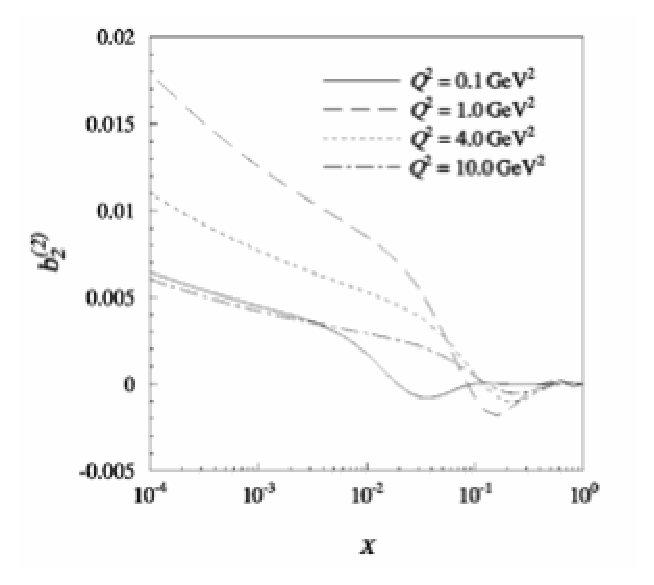
\includegraphics[width=0.40\textwidth]{figs/bora_jaffe_fig3.eps}
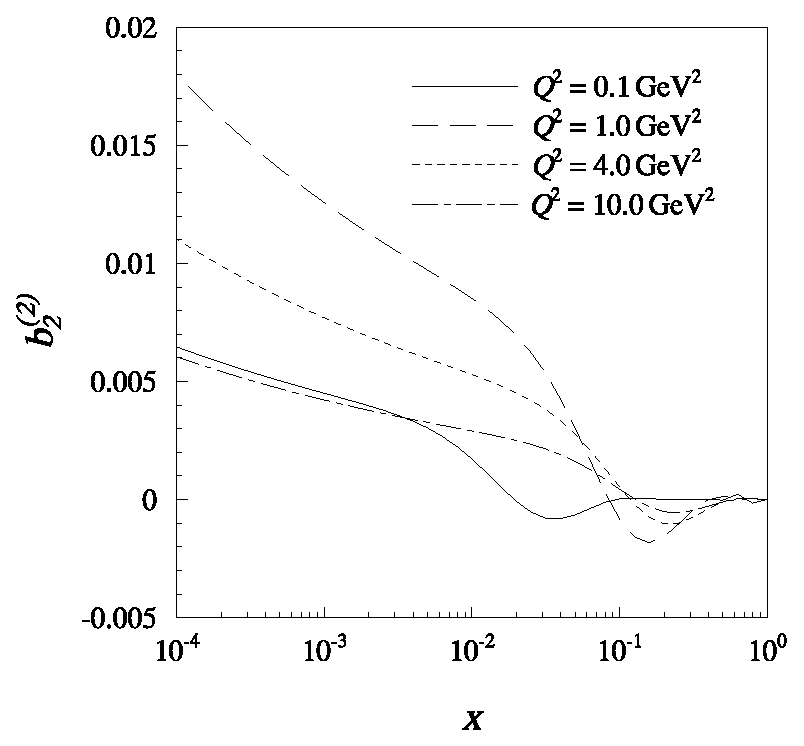
\includegraphics[width=0.3725\textwidth]{figs/bx.eps}
\hspace{0.3cm}
\includegraphics[width=0.45\textwidth]{figs/xb1_mstw_newmiller.eps}
\caption{\label{xb1_pred} Theoretical predictions. {\bf Left plot:} Double-scattering 
contribution to $b_2(x,Q^2)$ as a  function of $x$~\cite{Bora:1997pi}.  Note the strong $Q^2$ dependence at low x.
%($b_2 = b_2^{(1)}+b_2^{(2)}$). 
{\bf Right plot:} HERMES results~\cite{Airapetian:2005cb} compared to calculations 
from S.~Kumano~\cite{Kumano:2010vz} and from the one-pion exchange effects of 
G. Miller~\cite{Miller:1989nc,Miller_tmp}.}
\end{center}
\end{figure}

\begin{figure}
\begin{center}
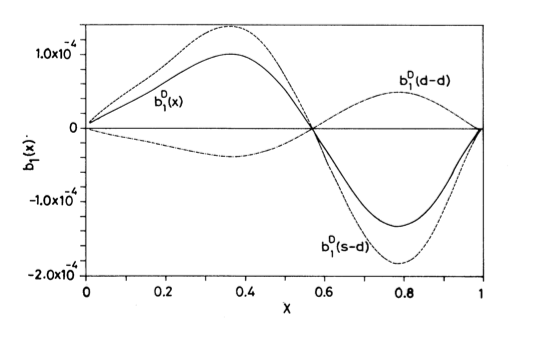
\includegraphics[width=0.45\textwidth]{figs/khan_pervez.eps}
\caption{\label{KHAN} Prediction for b$_1^D(x)$ (solid curve) from Ref.~\cite{Khan:1991qk}, the S-D contribution to b$_1^D(x)$ (dashed curve), and the D-D contribution to b$_1^D(x)$ (dot-dashed curve).  Note the vertical scale which would make the curve mostly indiscernible from zero in Fig.~\ref{xb1_pred} (right). {\it Reproduced from Ref.~\cite{Khan:1991qk}}.
}
\end{center}
\end{figure}
\subsubsection{Nuclear Pions}
In 1988, Miller also examined the tensor structure function $b_1$~\cite{Miller:1989nc}.
The basic mechanism is that the virtual photon hits an exchanged pion  which
is responsible for the binding of the deuteron. 
%The calculation depends on the choice of pion structure function which carries uncertainty. 
In this early calculation, the convention used by Miller for $b_1$ was different from that
used in the HERMES results and in Ref.~\cite{Kumano:2010vz}. A recent update to this  
calculation~\cite{Miller_tmp}, which uses a consistent convention and the pion structure
function from~\cite{Sutton:1991ay}, is shown in Fig.~\ref{xb1_pred}. The spread of the curve originates from the 
parameter $A_s=(.9 \pm 0.3)$ which governs the strength of the sea in the pion. 
Miller's calculation, similar to other `non-exotic' models, is unable to reproduce the trend of the HERMES data, and predicts very small values of $b_1(x)$ at intermediate and large $x$.
%These 
%numbers are all in qualitative agreement with the existing HERMES~\cite{Airapetian:2005cb} data, given their large error bars.
%Coherent-double scattering is expected to contribute also, but is not included in the Miller calculation. 
%Miller  specified that his mechanism is not the same as that, even though the HERMES 
%publication~\cite{Airapetian:2005cb} combined them together.

%In addition, at $x > 0.2$, a non-negligible value of $b_1^d$ is expected just through
%the conventional nuclear effects in the deuteron, Fermi motion and binding~\cite{Khan:1991qk}.
%\subsubsection*{Khan and Hoodbhoy}
\subsubsection{Convolution Model}
Khan and Hoodbhoy~\cite{Khan:1991qk} evaluated $b_1(x)$ in a convolution model with relativistic and binding energy corrections.  They use this to evaluate the effect of nuclear Fermi motion and binding on the deuteron structure functions.  They observe that for zero Fermi motion and binding $b_1^D(x)=0$.  
They also predict a small enhancement of $b_1$ in the region of $x\sim 0.3$, as seen in Fig.~\ref{KHAN}.  Note however, that the absolute scale of this predicted $b_1$ is 
$\mathcal{O}(10^{-4})$, while the HERMES data implies that the scale is more than an order of magnitude larger than this.

\subsubsection{Relativistic Calculation}
Umnikov~\cite{Umnikov:1996qv} calculated $b_1(x)$ and $b_2(x)$ within a covariant approach,
based on the relativistic convolution formalism for DIS and the  Bethe-Salpeter formalism 
for the deuteron bound state.  Fig.~\ref{UMNIKOV} sets the scale for $b_1(x)$ at the $10^{-3}$ level.  Both the relativistic and non-relativistic calculations are consistent with the CK sum rule (see Sec.~\ref{CKSEC}), although the nonrelativistic convolution model results in an incorrect behaviour of at low $x$.

\begin{figure}
\begin{center}
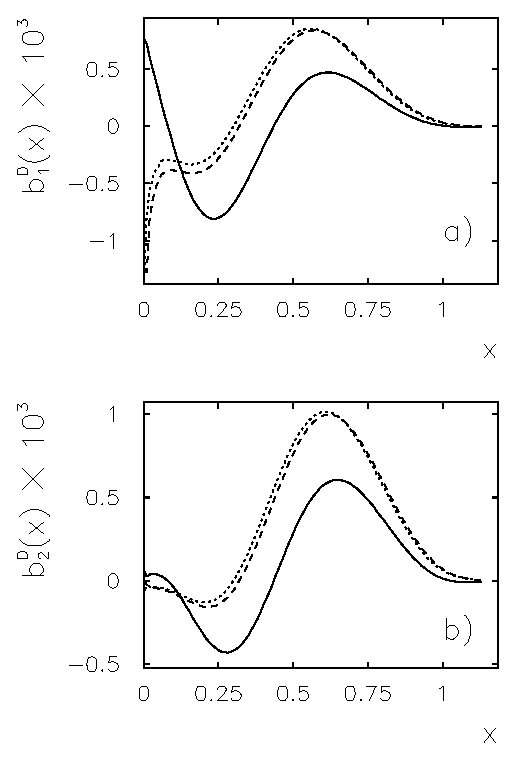
\includegraphics[width=0.3\textwidth]{figs/umnikov_b12.eps}
\caption{\label{UMNIKOV} Relativistic convolution calculation of $b_1^D(x)$ and $b_2^D(x)$.  Curves: BS - solid, Bonn - dotted, Bonn with cut -dashed.
{\it Reproduced from Ref.~\cite{Umnikov:1996qv}.}
}
\end{center}
\end{figure}


%
\subsubsection{Double-Scattering Effects}
Using Vector Meson Dominance (VMD), the authors of Ref.~\cite{Bora:1997pi} isolate the 
double-scattering contribution to $b_1$. The existence time of a vector meson can 
be described by the coherence length: %$\lambda$: 
\begin{eqnarray}
\lambda = \frac{Q^2}{M x (M_v^2 + Q^2)}
\end{eqnarray}
which is the length over which the vector meson propagates during the time $\Delta t 
= 1/\Delta E$. For significant shadowing or double scattering to occur, a minimum coherence length 
of $\approx$ 1.7 fm (the inter-nucleon separation) is required. At 
$x > 0.3$, the coherence length is only about the size of the nucleon, so double
scattering contributions are anticipated to be negligible. However, for $x \le 0.1$, 
double-scattering should be significant in $b_1$ behaving as $(1-x)^{2\delta}/x^{1+2\delta}$, 
where $\delta$ is determined from the soft pomeron intercept $\alpha_P(t=0) = 1 + \delta$.
The authors predicted a significant enhancement of $b_1$ at low $x$ ($\le$ 0.01) 
due to the quadrupole deformation of the deuteron, which is qualitatively confirmed by the
HERMES data.  See Fig.~\ref{HERMES_AZZ}.
%\begin{figure}[t]
%\begin{center}
%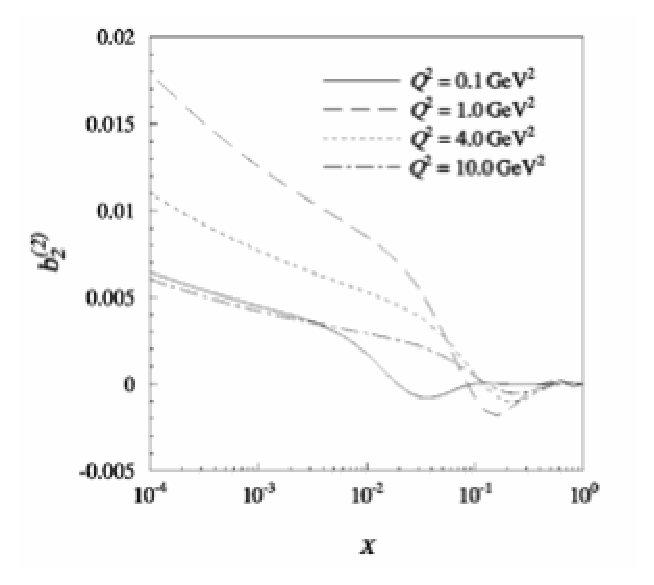
\includegraphics[width=0.5\textwidth]{figs/bora_jaffe_fig3.eps}
%\caption{\label{b2_bora} Double-scattering contribution $b_2^{(2)}(x,Q^2)$ in 
%function of $x$~\cite{Bora:1997pi} (where $2 x b_1 = b_2 = b_2^{(1)}+b_2^{(2)}$).}
%\end{center}
%\end{figure}

\subsubsection{Virtual Nucleon Approximation}
  %Following the approach of Ref.~\cite{Frankfurt:1983qs},
M. Sargsian~\cite{MISAK} recently calculated the tensor asymmetry $A_{zz}$ for deep inelastic scattering.   
%Within the  PWIA approximation in which parton distributions in the deuteron  are generated
%due to partons in proton and neutron, he predicts no significant tensor asymmetry except at
%very large x (quasi-elastic scattering) in which case the D-wave becomes important. See Fig.~\ref{PROJ}.
%
See Fig.~\ref{PROJ}.  In the approximation in which  only proton-neutron component of the deuteron is taken into account and  nuclear parton distributions
are generated through the convolution of partonic distribution of nucleon and deuteron density matrix (see e.g. Refs.~\cite{Frankfurt:1981mk,Sargsian:2001gu}), %       FS81,SSS},   
the deuteron structure function $b_1$ is related directly to the d-partial wave of the deuteron wave function~\cite{MISAK,Frankfurt:1981mk}.   %\cite{FS81,MS}.  
As a result,  this approximation predicts negligible  magnitude for $b_1$  for $x\le 0.6 $ due to small Fermi momenta involved  in the convolution integral. 
However, the predicted magnitude of $b_1$ is large at $x \ge 0.7$ where one expects substantial contribution from the d-waves due to 
high momentum component of the deuteron wave function involved in the convolution picture of DIS scattering off the deuteron.
In this case, $b_1$ is very sensitive to the relativistic description of the deuteron and its measurement can be used for checking 
the different approximations of high momentum  component of deuteron wave function.  

In the calculation presented, two Virtual Nucleon  and Light-Cone approximations are used to calculate the  tensor polarization for 
DIS scattering off the deuteron.  In both approximations only the proton-neutron component of the deuteron is taken into account.
In the Virtual Nucleon approximation, the covariant scattering amplitude is reduced  by estimating the spectator nucleon 
propagator at its on-energy shell in the lab frame of the deuteron.  Within this approximation the baryonic sum rule is satisfied while the 
momentum sum rule is not. The latter is due to the fact that part of the light cone momentum of the bound  virtual nucleon is lost to the 
unaccounted non-nucleonic degrees of freedom in the deuteron wave function.
In the light cone approximation the scattering amplitude is estimated the $E+p_z$ pole of the spectator nucleon on the light cone.
In this case the wave function is defined on the light-cone reference frame and it satisfies both baryon number and momentum sum rules.
For the detailed comparison  of these approximations, see Ref.~\cite{Sargsian:2001gu}.   %~\cite{SSS}.



\subsubsection{Fit to HERMES  Data}
Kumano~\cite{Kumano:2010vz} points out that the twist-2 structure functions $b_1$ and $b_2$ can be used to probe orbital angular momentum.  
He then extracts the tensor polarized quark and anti-quark distributions from a fit to the HERMES data~\cite{Airapetian:2005cb}. 
He finds that a non-negligible tensor polarization of the sea is necessary to reproduce the trend of
the data, as shown in Fig.~\ref{xb1_pred}. However, this conclusion has to be considered with caution due to the extended
$Q^2$ coverage (Fig.~\ref{HERMES_KIN}), and large uncertainty of each HERMES data point.
In particular, the author calls for better measurements of $b_1$ at large $x$ ($>0.2$), and further investigation of
the tensor structure functions in general.

\subsubsection{The Close-Kumano Sum Rule}
\label{CKSEC}
Following the formalism from the parton model in~\cite{Hoodbhoy:1988am}, Close and
Kumano~\cite{Close:1990zw} related the tensor structure function $b_1$ to the electric quadrupole
form factor of the spin-1 target through a sum rule\footnote{Efremov and Teryaev evidently proposed the same relation for
mesons in Ref.~\cite{Efremov:1981vs}.}:
\begin{eqnarray}
\int_0^1 dx~b_1(x)  & = &  - \frac{5}{12 M^2} \lim_{t \rightarrow 0}~t~F_Q(t)
                           + \frac{1}{9} \Big(\delta Q + \delta \bar{Q}\Big)_s \nonumber \\
                    & = & \frac{1}{9} \Big(\delta Q + \delta \bar{Q}\Big)_s  = 0 
\label{cksum}
\end{eqnarray}
where $F_Q(t)$ is the electric quadrupole form factor of a spin-1 hadron at the momentum squared $t$. 
The Close Kumano (CK) sum rule is satisfied in the case of an unpolarized sea. The authors note
that in nucleon-only models, the integral of $b_1$ is not sensitive to the
tensor-polarization of the sea, and consequently the sum rule is always true, even when the
deuteron is in a $D$-state.

The authors of Ref.~\cite{Khan:1991qk} calculated 
the first moment of $b_1(x)$ in a
version of the convolution model that incorporates relativistic and binding energy corrections.  They found a value of -6.65$\cdot 10^{-4}$, and
emphasize that deviations from this will serve as a good signature of exotic effects in the deuteron wave function.  Similarly, Ref.~\cite{Umnikov:1996qv} predicts $5\cdot 10^{-4}$ and  $3\cdot 10^{-5}$ for the relativistic and nonrelativistic calculation of Eq.~\ref{cksum}, respectively.




A truncated version of Eq.~\ref{cksum} was evaluated by the HERMES~\cite{Riedl:2005jq,Airapetian:2005cb} experiment and found to be:
\begin{eqnarray}
\int_{0.0002}^{0.85} b_1(x) dx = 0.0105 \pm 0.0034 \pm 0.0035
\end{eqnarray}
which possibly indicates a breaking of the Close-Kumano sum rule, and consequently a
tensor-polarized quark sea.  However, since the comparison is only at the two sigma level,  more precise data is needed for a true test.


%


\newpage
\subsection{Interest from Theorists}
%
During the preparation of this proposal, we contacted several theorists 
to gauge interest in a precision measurement of $b_1$.  The response was uniformly positive.  We 
provide some of their feedback for context.
%
%\vspace{0.5cm}
%{\bf S. Kumano (KEK and Tsukuba U.):}
%\vspace{0.5cm}
%{\bf M. Strikman (Penn. State U.) and M. Sargsian (FIU):}
%

\vspace{0.5cm}
\noindent
{\it 
%The tensor structure of the deuteron can be investigated in the deep
%inelastic region by measuring the structure function $b_1$, which
%should shed light on a new aspect of tensor-structure studies in
%terms of quark degrees of freedom instead of hadronic ones.
%There is a conventional approach for theoretically calculating $b_1$
%by quark distribution functions convoluted with nucleon momentum
%distributions in the deuteron including the $D$-state admixture.
%According to our experience on the nucleon-spin issue, such
%a conventional approach for high-energy spin physics would not work.
%In particular, 
It is known that $b_1$ is sensitive to dynamical aspects
of constituents with angular momenta. 
%
Measurements of $b_1$ could open
a new field of spin physics because this kind of spin physics has not
been explored anywhere else. The only experimental information came from
the HERMES collaboration; however, their data are not accurate enough
to find the $x$ dependence of $b_1$, especially at large $x$. 

It is an unique opportunity at JLab to develop this new field of spin physics.

%I think that your experiment should be an important one
%for opening a few field of hadron physics.
%so I hope that your proposal will be accepted.
}
\begin{flushright}{\bf S. Kumano (KEK)}\end{flushright}

\vspace{0.5cm}
\noindent
{\it I'm glad to hear that $b_1$ is not forgotten in all the excitement about other spin dependent 
effects.
%I don't have much to add to the existing discussion of $b_1$ in the literature. 
%If I remember correctly, 
%The hard thing is to distinguish a non-trivial contribution to $b_1$ (eg. 
%from 6 quark correlations in the deuteron) from the contribution from the deuteron d-wave.
}
%I 
%also remember a debate about a double scattering contribution.  I wrote a paper on that subject 
%with an Indian visitor to the CTP.  I believe our work was a follow-on to work by Nikolaev and 
%Schafer~\cite{Nikolaev:1996jy}.  I think these papers suggested large contributions to $b_1$ at 
%low x and low $Q^2$.}''
\begin{flushright}{\bf R. Jaffe (MIT)}\end{flushright}

\vspace{0.5cm}
\noindent{\it I am particularly interested in signatures of novel QCD effects in the deuteron. The tensor 
charge could be sensitive to hidden color (non-nucleonic) degrees of freedom at large $x$. It is
also interesting that antishadowing in DIS in nuclei is not universal but depends on the quark 
flavor and spin. One can use counting rules from PQCD to predict the $x \to 1$ dependence of the 
tensor structure function.}
\begin{flushright}{\bf S. Brodsky (SLAC)}\end{flushright}
 
\vspace{0.5cm}
\noindent{\it I am certainly interested in the experimental development to find the novel
QCD phenomena from the hidden color component of deuteron.}
\begin{flushright}{\bf Chueng-Ryong Ji (NCSU)}\end{flushright}

\vspace{0.5cm}
\noindent{\it You have finally piqued my interest in this subject...Surely this 
is of real interest the spin community!  I hope I might be able to say something coherent
about the partonic interpretation at some point--this of course is where my real interest lays.}
\begin{flushright}{\bf Leonard Gamberg (Penn State Berks)}\end{flushright}

\vspace{0.5cm}
\noindent{\it I find the proposal well written, well justified, sound, and exciting.}
\begin{flushright}{\bf Alessandro Bacchetta (Universita di Pavia)} \end{flushright}

